\documentclass[10pt]{beamer}

% Theme and style
\usetheme{metropolis}        % You can change this to e.g., CambridgeUS, Berlin, etc.
\usecolortheme{rose}  % Neutral color theme
\setbeamertemplate{navigation symbols}{}

% Packages
\usepackage{amsmath, amsfonts, amssymb}
\usepackage{graphicx}
\usepackage{booktabs}
\usepackage{dsfont}
\usepackage{xcolor}
\usepackage{subcaption}
\usepackage{natbib}

% Slide number position
\setbeamertemplate{footline}{
  \hfill
  \usebeamercolor[fg]{page number in head/foot}
  \usebeamerfont{page number in head/foot}
  \insertframenumber\,/\,\inserttotalframenumber\hspace{0.3cm}\vspace{0.1cm}
}

\setbeamertemplate{blocks}[rounded][shadow=true]

\newcommand{\Tc}{{\mathcal T}}
\newcommand{\fee}{\mathfrak{r}}
\newcommand{\mfT}{{\mathfrak{T}}}

\DeclareMathSymbol{\shortminus}{\mathbin}{AMSa}{"39}

% Title information
\title[]{Optimal Exit Time for Liquidity Providers in Automated Market Makers}
\author{Philippe Bergault\inst{\tiny{1}}, Sébastien Bieber\inst{\tiny{2}}, Leandro Sánchez-Betancourt\inst{\tiny{3}}}
\institute{
	\inst{1,2} Université Paris-Dauphine PSL,\inst{3} Oxford-Man Institute of Quantitative Finance.}
\date{London -- Paris Bachelier Workshop, November 2025}

\begin{document}

%------------------------------------------------
\begin{frame}
  \titlepage
\end{frame}

\section{Introduction}
%\begin{frame}{Cryptocurrency Ecosystem Insights}
%\textbf{Segmentation of the Cryptocurrency Market}\pause
%\vspace{1em}

%\begin{block}{Traditional Financial Exchanges \small{e.g., CME, Eurex, Cboe Digital}}
%Operate off-chain with stringent rules enforced by authorities (SEC, FCA, AMF).
%\end{block}\pause

%\begin{block}{Crypto-native Centralized Exchanges \small{e.g., Binance, Deribit, Coinbase}}
%Operate mostly off-chain with minimal oversight from financial authorities.
%\end{block}\pause

%\begin{block}{Fully Decentralized Applications \small{e.g., Uniswap, Aave, Morpho, dYdX}}
%Run directly on blockchain networks (Ethereum, Solana, Polygon) via \textbf{smart contracts}, using \textbf{oracles} for off-chain data.
%\end{block}

%\end{frame}

%------------------------------------------------

%\begin{frame}{Core Definitions}

%\begin{block}{Smart Contract}
%Self-executing program on the blockchain that runs when specific rules are met; results are irreversible and trackable.
%\end{block}

%\pause

%\begin{block}{Oracle}
%A service that connects smart contracts to external data, enabling secure access to off-chain information.
%\end{block}

%\pause

%\begin{block}{AMM}
%Protocol that lets users trade and provide liquidity directly through smart contracts, with prices determined by mathematical algorithms.
%\end{block}

%\end{frame}

%------------------------------------------------

\begin{frame}{Automated Market Makers (AMMs)}

\begin{block}{AMM}
Protocol that lets users trade and provide liquidity directly through smart contracts, with prices determined by mathematical algorithms.
\end{block}\pause

\textbf{Key Features:}\pause
\begin{itemize}
  \item Agents: Liquidity Providers (LP) deposit a pair of assets; Liquidity Takers (LTs) swap one asset against another.
  \item Price discovery: Uses pre-defined and public algorithms instead of order books or human market makers.
  \item Transparency: Liquidity in the pool is always publicly visible.
\end{itemize}

\begin{alertblock}{Note}
CFMMs are the most popular type of AMMs
\end{alertblock}

\end{frame}


\begin{frame}{Constant Function Market Makers (CFMM)}

\begin{block}{CFMM}
  CFMMs are characterized by a trading function $f: \mathbb{R}_+^* \times \mathbb{R}_+^* \to \mathbb{R}$.
  \begin{itemize}\setlength\itemsep{0.8em}
    \item If $q^0$ and $q^1$ are reserves of assets $0$ and $1$, a swap of $\Delta q^1$ coins of asset $1$ for $\Delta q^0$ coins of asset $0$ satisfies:
    $$f(q^0 - \Delta q^0, q^1 + \Delta q^1) = f(q^0, q^1)$$
  \end{itemize}
$\rightarrow$ The function $f(q^0, q^1)$ is preserved in a trade (ignoring transaction costs).
\end{block}\pause

\begin{exampleblock}{Constant Product Market Makers (CPMM)}
  The most common CFMM is the Constant Product Market Maker, where 
  $$f(q^0, q^1) = q^0 q^1$$
\end{exampleblock}

\end{frame}

%\begin{frame}{Extract of Existing Literature on AMM}
%  \begin{itemize}
%    \item \textbf{Main properties of CPMM:} \cite{angeris2021analysis}
%    \item \textbf{Decentralised liquidity pools and dynamic bonding curves for capital efficiency:} \cite{cartea2024strategic}
%    \item \textbf{Fee structures in an AMM:} \cite{evans2021optimal, cao2025structural, baggiani2025optimal, campbell2025optimal}
%    \item \textbf{Impermanent loss in an AMM:} \cite{milionis2022LVR}; \cite{canidio2023arbitrageurs}; \cite{cartea2023IL}; \cite{bergault2024automated}; %\cite{fukasawa2024model}
%    \item \textbf{Competition between limit order books and AMMs:} \cite{aoyagi2025coexisting, barbon2021quality, lehar2025decentralized}
%    \item \textbf{Static optimal exit time from an AMM:} \cite{zhu2025optimal}  
%   \end{itemize}
   
%\end{frame}

%------------------------------------------------

%\begin{frame}{Going beyond ...}
%\begin{block}{Key contribution of this paper:}
%  \begin{itemize}
%    \item Analysis of a dynamic optimal exit time for a LP in an AMM.
 %   \item Design of two numerical approach to solve the problem: an Euler scheme and a regression-based Longstaff--Schwartz algorithm.
 %   \item Calibration of the model and test the optimal strategy on real market data.
 % \end{itemize}
% \end{block}
%\end{frame}
%------------------------------------------------

\section{Model \& Problem Formulation}

\begin{frame}{Model Setup}

\begin{block}{Liquidity Pool Setup}\pause
\begin{itemize}
	\item A LP deposits a pair of assets $X$ (e.g., USDC) and $Y$ (e.g.; ETH) for a time horizon $T > 0$ into a liquidity pool with the CPMM function.\\ \pause
	\item We assume the existence of an external limit order book venue for trading $X$ and $Y$, where price formation occurs.\pause
	\item LTs arrive according to the counting processes $N^a$ and $N^b$.\pause
\end{itemize}
\end{block}

\begin{block}{Some notations}\pause
   \begin{itemize}
        \item $X_t$, $Y_t$: quantities of assets $X$ and $Y$ in the pool at time $t \leq T$, \pause
        \item $Z_t$: local price of $Y$ in terms of $X$ at time $t \leq T$, \pause
        \item $S_t$: external mid-price of asset $Y$ in terms of asset $X$ at time $t \leq T$,\pause
        \item $N_t^a$, $N_t^b$: number of liquidity taking buys, sells at time $t \leq T$,\pause
        \item $\xi$: trade size.
    \end{itemize}
\end{block}
\end{frame}


\begin{frame}{Dynamics of Reserves and Price}

\begin{block}{Dynamics of reserves $X$, $Y$, and local price $Z$}\pause
\footnotetext{\cite{cartea2024strategic}}
	\vspace{-1em}
    \begin{equation}
    \begin{aligned}
    \text{d} Y_t &= \xi \, \text{d} N^b_t - \xi \, \text{d} N^a_t, \\
    \text{d} X_t &= \left[\varphi_c(Y_{t\shortminus} + \xi) - \varphi_c(Y_{t\shortminus})\right] \, \text{d} N^b_t + \left[\varphi_c(Y_{t\shortminus} - \xi) - \varphi_c(Y_{t\shortminus})\right] \, \text{d} N^a_t, \\
    \text{d} Z_t &= \left[- \varphi_c'(Y_{t\shortminus} + \xi) + \varphi_c'(Y_{t\shortminus})\right] \, \text{d} N^b_t + \left[- \varphi_c'(Y_{t\shortminus} - \xi) + \varphi_c'(Y_{t\shortminus})\right] \, \text{d} N^a_t. \nonumber
    \end{aligned}
    \end{equation}
\end{block}\pause

\begin{alertblock}{Note} We define $\varphi_c(y) = \frac{c}{y}$ as the level function with constant depth $c$ throughout the trading horizon. The depth $c$ is determined at deposit inception and depends on the initial reserves ($c = X_0 Y_0$).
\end{alertblock}\pause

\begin{block}{Dynamics of External Mid-Price $S$}\pause
    \begin{equation}
    S_t = S_0 + \sigma W_t, \quad \text{where} \quad S_0 \in \mathbb{R}^+. \nonumber
    \end{equation}
\end{block}

\end{frame}

\begin{frame}{Designing Stochastic Intensities}
We suppose two types of LTs interacting with the liquidity pool:\pause
\vspace{-0.5em}
    \begin{itemize}
        \item \textbf{Arbitrageurs}: Look for profit from the price difference between the external venue and the AMM, thus the difference between $S$ and $Z$.\pause
        \item \textbf{Noise Traders}: They trade without regard to the price difference, usually for other purposes.\pause
    \end{itemize}

\begin{block}{Stochastic Intensities}\pause
        \begin{equation}
        \begin{aligned}
        \lambda^a_t = \bar{\lambda^a}(Z_{t^-}, S_t) &= \max\left\{ a_0, \, a_1 + a_2 \cdot (S_t - Z_{t^-}) \right\}, \\
        \lambda^b_t = \bar{\lambda^b}(Z_{t^-}, S_t) &= \max\left\{ a_0, \, a_1 + a_2 \cdot (Z_{t^-} - S_t) \right\}. \nonumber        
        \end{aligned}
        \end{equation}
        \begin{itemize}
            \item $a_0 > 0$: minimum base intensity.
            \item $a_1, a_2 \geq 0$: coefficients that modulate intensity based on price differences.
        \end{itemize}
    \end{block}

\end{frame}

\begin{frame}{Liquidity Provider Problem}

\begin{block}{Fees}\pause
Payments from LTs to the LP for executing trades as compensation for price risk and liquidity provision.
$$R_t= \int_0^t \fee(Y_{s\shortminus}) \left(\text{d} N^b_s + \text{d} N^a_s \right) \quad \text{with} \quad \fee : \mathbb{R_+} \rightarrow \mathbb{R_+}.$$
\end{block}

\begin{block}{Impermanent Loss (IL)}\pause
Reduction in value a LP experiences when the prices of the assets in the pool change, compared to simply holding those assets outside the pool.
$$\text{IL}_t := -\big[ X_t + Y_t S_t - (X_0 + Y_0 S_t) \big] = -\Big[ \underbrace{X_t - X_0}_{P^X_t} + S_t \underbrace{(Y_t - Y_0)}_{P^Y_t} \Big].$$
\end{block}\pause

\begin{alertblock}{Note}
We consider the case of a LP who owns the entire liquidity available in the AMM and that $\fee$ has linear growth.
\end{alertblock}

\end{frame}

\begin{frame}{Liquidity Provider Problem}

\begin{block}{LP's optimal problem}
The LP wants to maximise her fee revenues while minimizing her IL.\\ \quad \\
Let $\Tc_{t,T}$ be set of stopping times taking values in $[t,T]$, and $\Tc := \Tc_{0,T}$. \\ \quad \\
The LP optimal problem is: \\
$$\sup_{\tau \in \mathcal{T}} \mathbb{E}\Big[\underbrace{P^X_\tau + S_\tau P^Y_\tau}_{-\text{IL}_\tau} + R_\tau \Big].$$
\end{block}
\end{frame}

\begin{frame}{Value function and Dynamic Programming Principle}
%We write $-\text{IL}_t+R_t$ as
%\begin{equation}
%\begin{aligned}
%    P_t^X + S_t P_t^Y + R_t &= \displaystyle\int_0^t \overbrace{\left(\varphi_c(Y_{s^\shortminus} + \xi) - \varphi_c(Y_{s^\shortminus}) + \xi S_s + \fee(Y_{s^\shortminus})\right)}^{:=\beta^b(Y_{s\shortminus},S_s)} \text{d} N_s^b \\
%    &\quad + \displaystyle\int_0^t \underbrace{\left( \varphi_c(Y_{s^\shortminus} - \xi) - \varphi_c(Y_{s^\shortminus}) - \xi S_s + \fee(Y_{s^\shortminus}) \right)}_{:=\beta^a(Y_{s\shortminus},S_s)} \text{d} N_s^a. \nonumber
%\end{aligned}
%\end{equation}

%We define the value function $v$ for this optimal stopping time problem as the following:
%\begin{equation}
%\begin{aligned}
%v :\quad & [0,T] \times Q \times \mathbb{R} \longrightarrow \mathbb{R}, \\
%& (t, y, S) \longmapsto \sup_{\tau \in \mathcal{T}_{t,T}} \mathbb{E} \Bigg[ \int_{t}^{\tau}
%\bigg\{
%  \beta^b\big(Y^{t,y}_{s\shortminus}, S^{t,S}_s\big)\,\lambda^b_s\, + \beta^a\big(Y^{t,y}_{s\shortminus}, S^{t,S}_s\big)\,\lambda^a_s\,
%\bigg\} \,\mathrm{d}s \Bigg]. \nonumber
%\end{aligned}
%\end{equation}

We define the value function $v$ for this optimal stopping time problem as the following:
\begin{equation}
\scalebox{0.9}{$
\begin{aligned}
v:\, & [0,T] \times Q \times \mathbb{R} \longrightarrow \mathbb{R}, \\
& (t, y, S) \longmapsto \sup_{\tau \in \mathcal{T}_{t,T}} \mathbb{E} \Bigg[ \int_{t}^{\tau} \bigg\{\overbrace{\left(\varphi_c(Y^{t,y}_{s^\shortminus} + \xi) - \varphi_c(Y^{t,y}_{s^\shortminus}) + \xi S^{t,S}_s + \fee(Y^{t,y}_{s^\shortminus})\right)}^{:=\beta^b(Y^{t,y}_{s\shortminus},S^{t,S}_s)}\,\lambda^b_s\, \\
& \quad \quad \quad \quad \quad \quad \quad \quad \quad + \underbrace{\left( \varphi_c(Y^{t,y}_{s^\shortminus} - \xi) - \varphi_c(Y^{t,y}_{s^\shortminus}) - \xi S^{t,S}_s + \fee(Y^{t,y}_{s^\shortminus}) \right)}_{:=\beta^a(Y^{t,y}_{s\shortminus},S^{t,S}_s)}\,\lambda^a_s\,
\bigg\} \,\mathrm{d}s \Bigg]. \nonumber
\end{aligned}$}
\end{equation}\pause
\vspace{-0.5em}
\begin{block}{Dynamic Programming Principle}\pause
Let $(t,y,S) \in [0,T) \times Q \times \mathbb{R}$, then for all $\theta \in \mathcal{T}_{t,T}$ we have
\vspace{-0.5em}
    \begin{equation}
    \begin{aligned}
        v(t, y, S) = & \, \sup_{\tau \in \Tc_{t,T}} \mathbb{E}\bigg[\int_{t}^{\tau \wedge \theta}  \left[\, \beta^b(Y^{t,y}_{u\shortminus},S^{t,S}_u) \lambda^b_u +  \, \beta^a(Y^{t,y}_{u\shortminus}, S^{t,S}_u)\lambda^a_u \right] \text{d} u \bigg. \nonumber \\
        & \qquad \qquad \qquad \qquad \qquad \qquad \qquad + \mathds{1}_{\{\tau \geq \theta\}}v(\theta, Y^{t, y}_{\theta}, S^{t, y}_{\theta}) \bigg. \bigg] \nonumber.
    \end{aligned}
    \end{equation}
\end{block}

\end{frame}

\begin{frame}{Hamilton--Jacobi--Bellman Quasi--Variational Equation}
\begin{block}{HJB QVI}\pause
\begin{equation}
\begin{aligned}
        0 = \min\bigg\{& -\frac{\partial}{\partial t} v(t, y, S) \, - \frac{1}{2} \sigma^2 \frac{\partial^2}{\partial S^2} v(t, y, S) \, \\
        & - \bar{\lambda}^b(y, S) \big[ \beta^b(y,S) + v(t, y +\xi, S) - v(t, y, S) \big] \, \nonumber \\
        & - \bar{\lambda}^a(y, S) \big[ \beta^a(y,S) + v(t, y - \xi, S) - v(t, y, S) \big]\,  , \\ 
        & \, v(t,y,S) \bigg\} \qquad \text{on } [0,T) \times  Q \times \mathbb R, \nonumber \\
\end{aligned}
\end{equation}
with terminal condition $v(T,y,S)=0$ for all $(y,S) \in Q \times \mathbb R$.
\end{block}\pause

\begin{alertblock}{Note}
The problem is composed of two state variables, which makes it tractable for numerical simulation.
\end{alertblock}

\end{frame}

\section{Numerical Simulation}
\begin{frame}{Iterative solving methods}

\begin{block}{Euler method}\pause
The HJB QVI combines diffusion and jump terms. At each time step $\delta$, jump terms are treated explicitly, then diffusion is updated implicitly.
\end{block}\pause

\begin{block}{Recursive scheme for Longstaff--Schwartz method}\pause
We can approximate the solution numerically by leveraging the DPP at each time step $\delta$:
\begin{equation}
\begin{aligned}
    \hat{v}(t,y,S) = & \max \Bigg\{ \mathbb{E} \left[ \int_{t}^{t+\delta} \left\{ 
    \beta^b\left(Y^{t,y}_{s^-}, S^{t,S}_s\right) \, \lambda^b_s \, + \beta^a\left(Y^{t,y}_{s^-}, S^{t,S}_s\right) \, \lambda^a_s \, \right\} \, \text{d}s \right. \nonumber \\
    & \left.  + \, \hat{v}\left(t+\delta, Y_{t+\delta}^{t, y}, S_{t+\delta}^{t, S}\right) \right], 0 \Bigg\}, \nonumber
\end{aligned}
\end{equation}
with the terminal condition $\hat{v}(T,y,S)=0$.
\end{block}

\end{frame}

\begin{frame}{Comparison between Euler and Longstaff--Schwartz methods}
\begin{figure}[H]
    \centering
    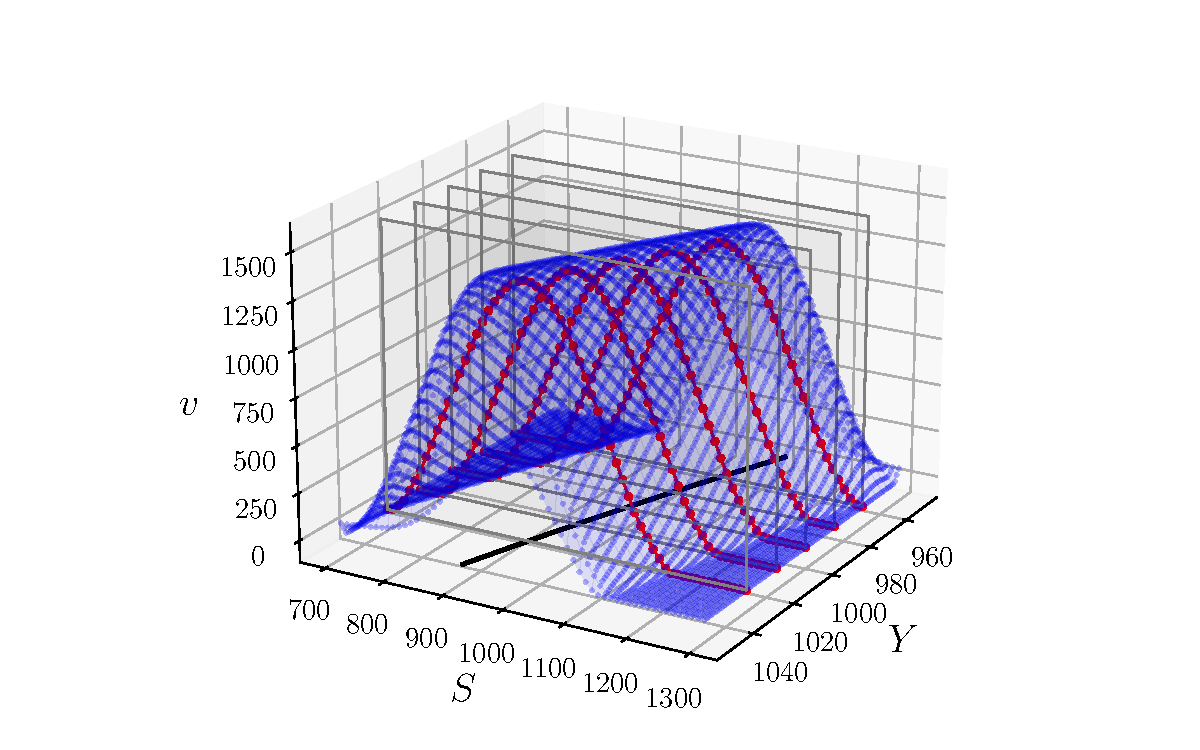
\includegraphics[width=0.49\linewidth]{../code/figures/3d-plot-euler-vs-ls-0.pdf}
    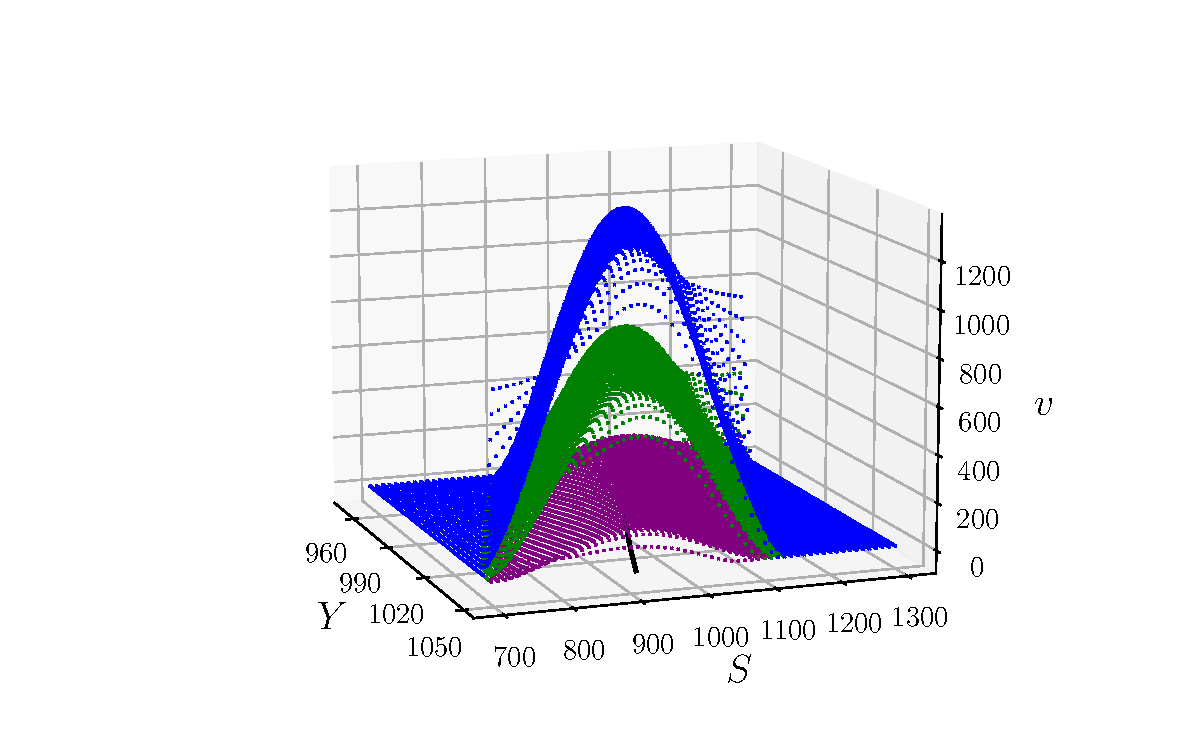
\includegraphics[width=0.49\linewidth]{../code/figures/3d-plot-euler-time_factor-0-05-09.pdf}
    \caption{Left: value function $v$ at $t = 0$ computed with the Euler method (blue surface) and Longstaff--Schwartz algorithm (red slices) with the black curve in the $S\text{-}Y$ plane representing states where $S = Z$. Right: Euler method value function at $t = 0$ (blue), $t = 0.5$ (green), and $t = 0.9$ (purple).}
\end{figure}
\vspace{-1em}
\begin{alertblock}{Note}
Fictitious parameters are used to ensure the stability of the Euler scheme.
\end{alertblock}

\end{frame}

\begin{frame}{Calibration on real market data}
\begin{exampleblock}{Market simulator}
\begin{itemize}
    \item Asset $X$: \textbf{USDC}, Asset $Y$: \textbf{ETH}
    \item Initial exchange rate: $S_0 = Z_0 = \textbf{2820}\,\$$
    \item Initial reserve: $Y_0 = \textbf{50,000}\;\text{ETH}$, $X_0 = Y_0 Z_0\,\$$
    \item Volatility: $\sigma = \textbf{0.0569}\,S_0\,\$ \cdot \text{day}^{-1/2}$
    \item Intensities: $a_0 = \textbf{1}\;\text{day}^{-1}$, $a_1 = \textbf{10}\;\text{day}^{-1}$, $a_2 = \textbf{10}\;\$^{-1}\cdot\text{day}^{-1}$
    \item Trade size: $\xi = \textbf{100}$
    \item Fees: $\fee = \textbf{0.01} \times \xi \times S_0$
    \item Horizon: $T = \textbf{1}\;\text{day}$
\end{itemize}

\end{exampleblock}

\begin{alertblock}{Note}
We use market data from \cite{aqsha2025equilibrium}, calibrated with Binance and Uniswap V2 ETH-USDC data from January to April 2022.
\end{alertblock}

\end{frame}

\begin{frame}{Sample path for liquidity pool price and reserve}
\begin{figure}[H]
    \centering
    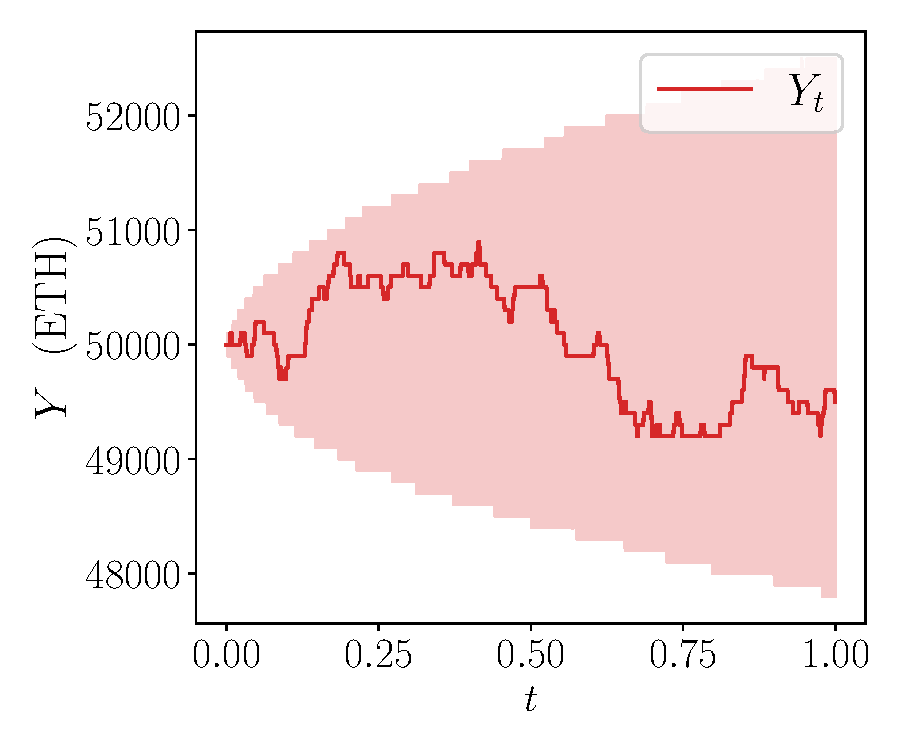
\includegraphics[width=0.49\linewidth]{../code/figures/Y-paths.pdf}
    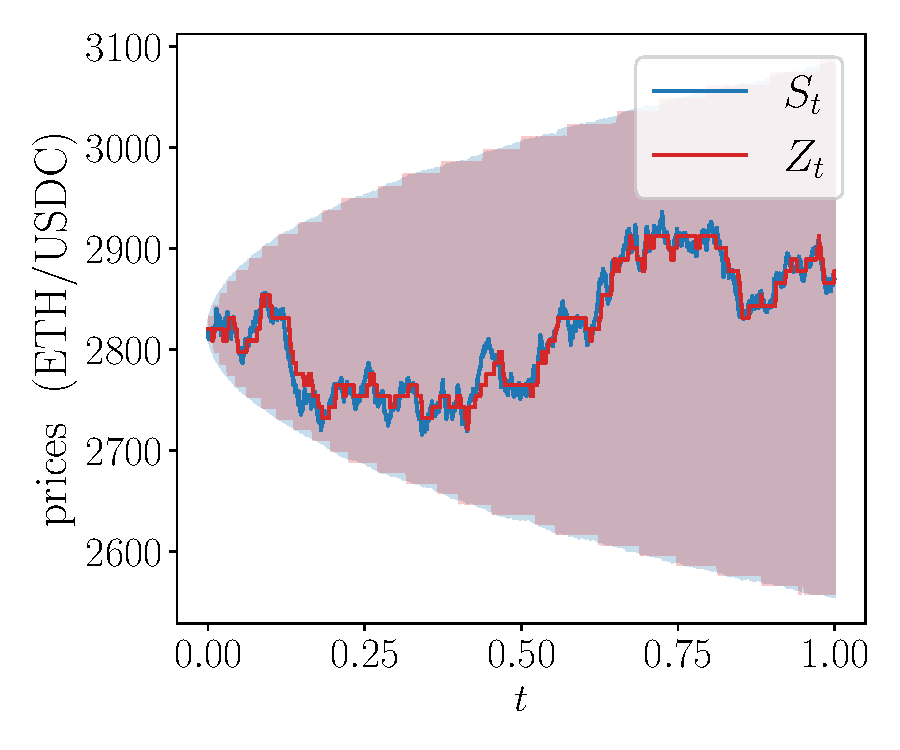
\includegraphics[width=0.49\linewidth]{../code/figures/S-Z-paths.pdf}
    \caption{Sample paths for the inventory process $Y_t$ (ETH) and the price processes $S_t$ and $Z_t$. All processes are accompanied by the running quantiles (5\% and 95\%) across time.}
\end{figure}

\end{frame}

\begin{frame}{Impact of volatility changes}
\begin{table}[H]
    \centering
    \begin{tabular}{l|rrr}
\hline
\hline
$\sigma_{\mathrm{new}}$ & $\mathbb{E}[\tau]$ & $\mathbb{E}[R_\tau]$ & $\mathbb{E}[\mathrm{IL}_\tau]$ \\
\hline
\hline
$\sigma$/5 & 1.00 (0.00) & 161,765 (22,320) & 4,364 (6,419) \\
$\sigma$/4 & 1.00 (0.00) & 168,343 (22,217) & 6,912 (10,024) \\
$\sigma$/3 & 1.00 (0.00) & 181,148 (21,806) & 12,422 (17,830) \\
$\sigma$/2 & 1.00 (0.00) & 210,406 (22,535) & 28,177 (40,154) \\
$\sigma$ & 1.00 (0.01) & \textcolor{red}{316,222 (26,930)} & 112,635 (157,844) \\
$2\,\sigma$ & 0.51 (0.27) & 273,003 (144,005) & \textcolor{red}{202,999 (372,645)} \\
$3\,\sigma$ & 0.01 (0.01) & 3,599 (9,363) & 2,449 (13,042) \\
$4\,\sigma$ & 0.00 (0.00) & 1,794 (3,984) & 1,304 (7,411) \\
$5\,\sigma$ & 0.00 (0.00) &\textcolor{blue}{532 (1,198)} & \textcolor{blue}{420 (1,401)} \\
\hline
\end{tabular}
    \caption{Summary statistics for the expected (i) exit time,\footnotemark[1] (ii) fees collected, and (iii) impermanent loss, as $\sigma$ varies. Mean values (with standard deviation in parenthesis) across 10,000 simulations.}
\footnotetext[1]{$\tau=T=1$ if the LP does not exit the pool before $T$.}
\end{table}

\end{frame}

\begin{frame}{Impact of fees changes}

Higher fees discourage LTs activity, so set $\tilde{a_i}=a_i \,e^{-\kappa(\tilde\fee - \fee)},\, i\in\{0,1,2\}$ to accurately evaluate the effect of fees.

\begin{table}%[H]
    \centering
    \begin{tabular}{l|rrr}
\hline
\hline
$\fee_{\mathrm{new}}$ & $\mathbb{E}[\tau]$ & $\mathbb{E}[R_\tau]$ & $\mathbb{E}[\mathrm{IL}_\tau]$ \\
\hline
\hline
$\fee$/5 & 0.01 (0.01) & \textcolor{blue}{373 (750)} & \textcolor{blue}{173 (1,308)} \\
$\fee$/4 & 0.04 (0.05) & 3,027 (5,099) & 2,239 (11,377) \\
$\fee$/3 & 0.11 (0.12) & 12,578 (14,578) & 8,437 (35,736) \\
$\fee$/2 & 0.96 (0.09) & 166,560 (20,956) & 105,643 (141,534) \\
$\fee$ & 1.00 (0.01) & 316,222 (26,930) & \textcolor{red}{112,635 (157,844)} \\
$2\,\fee$ & 1.00 (0.00) & 530,160 (50,735) & \textcolor{red}{113,269 (161,299)} \\
$3\,\fee$ & 1.00 (0.00) & 670,137 (71,973) & \textcolor{red}{113,126 (161,712)} \\
$4\,\fee$ & 1.00 (0.00) & 755,901 (91,748) & \textcolor{red}{112,825 (161,819)} \\
$5\,\fee$ & 1.00 (0.00) & \textcolor{red}{802,518 (109,834)} & \textcolor{red}{112,407 (161,782)} \\
\hline
\end{tabular}
    \caption{Summary statistics for the expected (i) exit time, (ii) fees collected, and (iii) impermanent loss, as $\fee$ varies.  Mean values (with standard deviation in parenthesis) across 10,000 simulations.}
\end{table}
\end{frame}

\begin{frame}{Impact of fees changes}

\begin{figure}[H]
    \centering
    %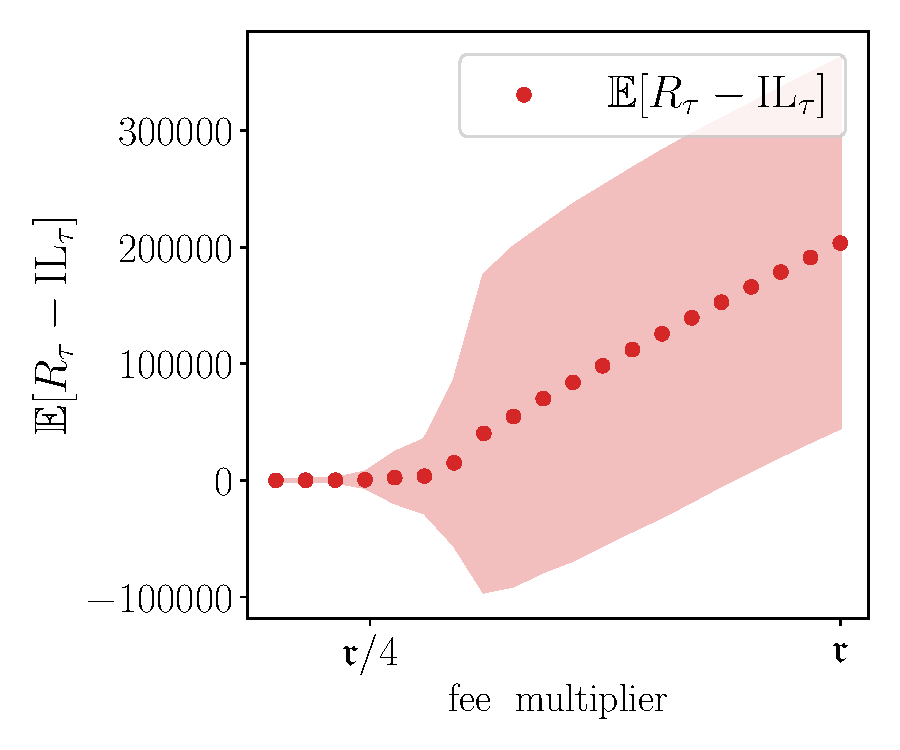
\includegraphics[width=0.45\linewidth]{../code/figures/fee-multiplier-and-performance_zoomed.pdf}    
    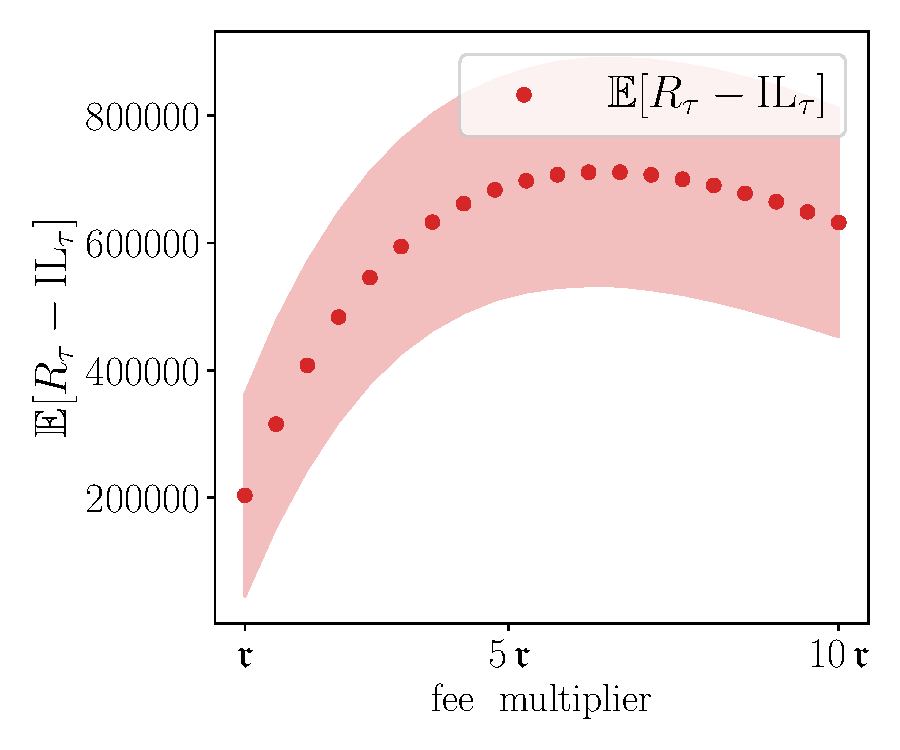
\includegraphics[width=0.6\linewidth]{../code/figures/fee-multiplier-and-performance.pdf}
    \caption{Relationship between $\fee$ and performance, measured through  $\mathbb{E}[R_\tau - \mathrm{IL}_\tau]$. The coloured area shows one standard deviation around the mean.}
\end{figure}

%Left panel is zoomed in for $(\fee/10,\fee]$ whereas the right  panel shows $(\fee, 10\,\fee]$.

\end{frame}

\begin{frame}{Impact of intensity changes ($a_1$)}
\begin{table}[H]
    \centering
    \begin{tabular}{l|rrr}
\hline
\hline
$a_1^{\mathrm{new}}$ & $\mathbb{E}[\tau]$ & $\mathbb{E}[R_\tau]$ & $\mathbb{E}[\mathrm{IL}_\tau]$ \\
\hline
\hline
$a_1$/5 & 1.00 (0.01) & \textcolor{blue}{296,407 (26,305)} & \textcolor{red}{112,619 (157,946)} \\
$a_1$/4 & 1.00 (0.01) & 297,518 (26,328) & \textcolor{red}{112,633 (157,824)} \\
$a_1$/3 & 1.00 (0.01) & 299,641 (26,392) & \textcolor{red}{112,652 (158,199)} \\
$a_1$/2 & 1.00 (0.01) & 303,577 (26,514) & \textcolor{red}{112,625 (157,865)} \\
$a_1$ & 1.00 (0.01) & 316,222 (26,930) & \textcolor{red}{112,635 (157,844)} \\
$2\,a_1$ & 1.00 (0.01) & 343,925 (27,871) & \textcolor{red}{112,757 (158,040)} \\
$3\,a_1$ & 1.00 (0.01) & 373,822 (29,214) & \textcolor{red}{112,910 (158,749)} \\
$4\,a_1$ & 1.00 (0.01) & 406,551 (30,439) & \textcolor{red}{112,767 (159,015)} \\
$5\,a_1$ & 1.00 (0.01) & \textcolor{red}{441,710 (31,530)} & \textcolor{red}{112,592 (158,793)} \\
\hline
\end{tabular}
    \caption{Summary statistics for the expected (i) exit time, (ii) fees collected, and (iii) impermanent loss, as $a_1$ varies. Mean values (with standard deviation in parenthesis) across 10,000 simulations. }
\end{table}
\end{frame}

\begin{frame}{Impact of intensity changes ($a_2$)}
\begin{table}[H]
    \centering
    \begin{tabular}{l|rrr}
\hline
\hline
$a_2^{\mathrm{new}}$ & $\mathbb{E}[\tau]$ & $\mathbb{E}[R_\tau]$ & $\mathbb{E}[\mathrm{IL}_\tau]$ \\
\hline
\hline
$a_2$/5 & 0.86 (0.21) & \textcolor{blue}{118,244 (33,981)} & \textcolor{blue}{83,734 (127,349)} \\
$a_2$/4 & 0.93 (0.13) & 142,756 (27,971) & 95,493 (139,173) \\
$a_2$/3 & 0.98 (0.07) & 173,770 (24,588) & 104,549 (148,242) \\
$a_2$/2 & 0.99 (0.03) & 216,953 (24,307) & 110,222 (153,239) \\
$a_2$ & 1.00 (0.01) & 316,222 (26,930) & 112,635 (157,844) \\
$2\,a_2$ & 1.00 (0.01) & 476,493 (31,957) & 113,284 (158,588) \\
$3\,a_2$ & 1.00 (0.01) & 618,447 (36,240) & 113,564 (159,533) \\
$4\,a_2$ & 1.00 (0.01) & 750,774 (40,318) & 113,758 (160,513) \\
$5\,a_2$ & 1.00 (0.00) & \textcolor{red}{878,099 (43,924)} & \textcolor{red}{113,789 (160,830)} \\
\hline
\end{tabular}
    \caption{Summary statistics for the expected (i) exit time, (ii) fees collected, and (iii) impermanent loss, as $a_2$ varies. Mean values (with standard deviation in parenthesis) across 10,000 simulations.}
\end{table}
\end{frame}

\section{Conclusion}
\begin{frame}{\,}

\textbf{Key Takeaway}\pause
\begin{itemize}
	\item LPs remain in the pool when fee income is greater than potential impermanent loss, particularly when volatility is low, fees are high, or trading activity is high.\pause
	\item Large price dislocations cause LPs to exit before arbitrageurs realign prices, to avoid incurring large impermanent loss.\pause
\end{itemize}

\textbf{Future research}\pause
\begin{itemize}
	\item Investigate how transaction costs and priority gas fees affect the competition between LPs and arbitrageurs.\pause
	\item Extend this framework to concentrated liquidity pools (e.g.; Uniswap v3)
\end{itemize}

\end{frame}
%------------------------------------------------

\begin{frame}[allowframebreaks]{}
    \frametitle{}  % Remove the frame title
    \renewcommand{\bibname}{}  % Remove the default "References" title
    \bibliographystyle{apalike}
    \bibliography{references}
\end{frame}


\end{document}
